\documentclass[a4 paper]{article}
% Set target color model to RGB
\usepackage[inner=1.5cm,outer=1.5cm,top=2.5cm,bottom=2.5cm]{geometry}
\usepackage{setspace}
\usepackage[rgb]{xcolor}
\usepackage{verbatim}
\usepackage{amsgen,amsmath,amstext,amsbsy,amsopn,tikz,amssymb,tkz-linknodes}
\usepackage{fancyhdr}
\usepackage[colorlinks=true, urlcolor=blue,  linkcolor=blue, citecolor=blue]{hyperref}
\usepackage[colorinlistoftodos]{todonotes}
\usepackage{rotating}
%\usetikzlibrary{through,backgrounds}
\hypersetup{%
pdfauthor={Arman Shokrollahi},%
pdftitle={Homework},%
pdfkeywords={Tikz,latex,bootstrap,uncertaintes},%
pdfcreator={PDFLaTeX},%
pdfproducer={PDFLaTeX},%
}
%\usetikzlibrary{shadows}
\usepackage[francais]{babel}
\usepackage{booktabs}
\newcommand{\ra}[1]{\renewcommand{\arraystretch}{#1}}

      \newtheorem{thm}{Theorem}[section]
      \newtheorem{prop}[thm]{Proposition}
      \newtheorem{lem}[thm]{Lemma}
      \newtheorem{cor}[thm]{Corollary}
      \newtheorem{defn}[thm]{Definition}
      \newtheorem{rem}[thm]{Remark}
      \numberwithin{equation}{section}

\newcommand{\homework}[6]{
   \pagestyle{myheadings}
   \thispagestyle{plain}
   \newpage
   \setcounter{page}{1}
   \noindent
   \begin{center}
   \framebox{
      \vbox{\vspace{2mm}
    \hbox to 6.28in { {\bf\hfill} }
       \vspace{6mm}
       \hbox to 6.28in { {\Large \hfill #1 (#2)  \hfill} }
       \vspace{6mm}
       \hbox to 6.28in { {\it Instructor: #3 \hfill Student: #5} }
       %\hbox to 6.28in { {\it TA: #4  \hfill #6}}
      \vspace{2mm}}
   }
   \end{center}
   \markboth{#5 -- #1}{#5 -- #1}
   \vspace*{4mm}
}

\newcommand{\bbF}{\mathbb{F}}
\newcommand{\bbX}{\mathbb{X}}
\newcommand{\bI}{\mathbf{I}}
\newcommand{\bX}{\mathbf{X}}
\newcommand{\bY}{\mathbf{Y}}
\newcommand{\bepsilon}{\boldsymbol{\epsilon}}
\newcommand{\balpha}{\boldsymbol{\alpha}}
\newcommand{\bbeta}{\boldsymbol{\beta}}
\newcommand{\0}{\mathbf{0}}

\begin{document}
\homework{Actividad \#2}{Efem\'erides}{Carlos Liz\'arraga Celaya}{}{Antonio Cota Rodr\'iguez}{}

\section*{Introducci\'on}
\subsection*{Efem\'erides}
En el estudio de los cuerpos celestes, una efem\'erides, efem\'eride o efemeris es una tabla de valores que da las posiciones de los objetos astron\'o\'omicos en el cielo en un momento o momentos dados. Aunque fue tambi\'e\'en una de las primeras aplicaciones de las computadoras mec\'a\'anicas, el t\'e\'ermino efem\'erides contin\'ua aplic\'andose generalmente a una simple tabla impresa.

\subsection*{Interpolaci\'on}
En el subcampo matem\'atico del an\'alisis num\'erico, se denomina interpolaci\'on a la obtenci\'on de nuevos puntos partiendo del conocimiento de un conjunto discreto de puntos.\\

En ingenier\'ia y algunas ciencias es frecuente disponer de un cierto n\'umero de puntos obtenidos por muestreo o a partir de un experimento y pretender construir una funci\'on que los ajuste.\\

Otro problema estrechamente ligado con el de la interpolaci\'on es la aproximaci\'on de una funci\'on complicada por una m\'as simple. Si tenemos una funci\'on cuyo c\'alculo resulta costoso, podemos partir de un cierto n\'umero de sus valores e interpolar dichos datos construyendo una funci\'on m\'as simple. En general, por supuesto, no obtendremos los mismos valores evaluando la funci\'on obtenida que si evaluamos la funci\'on original, si bien dependiendo de las caracter\'isticas del problema y del m\'etodo de interpolaci\'on usado la ganancia en eficiencia puede compensar el error cometido.\\

En todo caso, se trata de, a partir de $n$ parejas de puntos $(x_{k},y_{k})$, obtener una función $f$ que verifique 

$$f(x_{k}) = y_{k}, \quad k=1,\cdots,n$$

\section*{Programa}

En esta actividad aprenderemos un poco del proceso de encontrar una funci\'on que interpole todos los puntos, apoyados en la funci\'on {\it scipy.interpolate} de Python.

Con base en el siguiente c\'odigo:

\begin{verbatim}

import numpy as np
import matplotlib.pyplot as plt
from scipy.interpolate import interp1d

# Original "data set" --- 21 random numbers between 0 and 1.
x0 = np.linspace(-1,1,21)
y0 = np.random.random(21)

plt.plot(x0, y0, 'o', label='Data')

# Array with points in between those of the data set for interpolation.
x = np.linspace(-1,1,101)

# Available options for interp1d
options = ('linear', 'nearest', 'zero', 'slinear', 'quadratic', 'cubic', 10)

for o in options:
    f = interp1d(x0, y0, kind=o)    # interpolation function
    plt.plot(x, f(x), label=o)      # plot of interpolated data

plt.legend()
plt.show()
\end{verbatim}

Este programa nos da una gr\'afica de datos interpolados de distintas formas (cuadr\'atica, c\'ubica, etc.) para n\'umeros aleatorios, la gr\'afica es la siguiente

\vspace{0.5cm}

\begin{figure}[!ht]
  \centering
      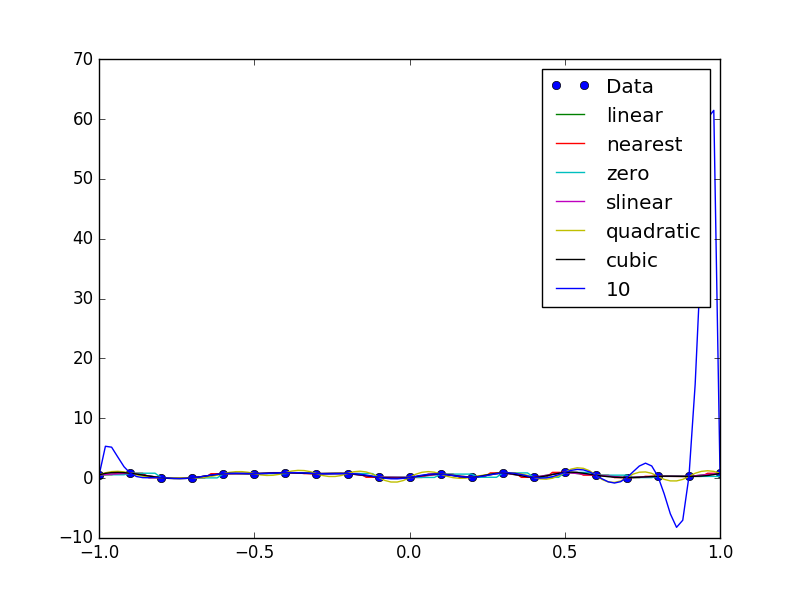
\includegraphics[width=8cm, height=6cm]{ejemplo.png}
  \caption{Ejemplo}
\end{figure}

\vspace{0.5cm}

A continuaci\'on se modficar\'a el c\'odigo anterior para realizar una interpolaci\'on lineal, cuadr\'atica y c\'ubica de los siguientes casos:\\

\begin{itemize}
\item Dados 10 puntos aleatorios entre $x=0$ y $x=3$ para la función $f(x) = \sin(2x)$.
\item Dados 20 puntos aleatorios entre $x=-10$ y $x=10$ para la función $f(x) = \sin(x)/x$.
\item Dados 16 puntos aleatorios entre $x=-3$ y $x=3$ para la función $f(x) = x^{2}\sin(2x)$
\item Dados 12 puntos aleatorios entre $x=-2$ y $x=2$ para la función f(x) = $x^{3}\sin(3x)$
\end{itemize}

\section{$\sin(2x)$}

El programa para interpolar esta funci\'on es el siguiente:

\begin{verbatim}
import numpy as np
import matplotlib.pyplot as plt
from scipy.interpolate import interp1d

# Original "data set" --- 10 random numbers between 0 and 3.
xn = np.random.random(10)
x = xn*3
# Original "Data-set"
y = np.sin(2*x)

plt.plot(x, y, 'o', label='Data')

# Array with points in between those of the data set for interpolation.
xnew = np.linspace(min(x), max(x), 10000)
# Available options for interp1d
options =('linear','quadratic','cubic')
for o in options:
    f = interp1d(x, y, kind=o)    # interpolation function
    plt.plot(xnew, f(xnew), label=o)  # plot of interpolated data
    
plt.legend(['data', 'linear', 'quadratic', 'cubic'], loc='best')
plt.show()
\end{verbatim}

Obtenemos la gr\'afica 

\vspace{0.5cm}

\begin{figure}[!ht]
  \centering
      \includegraphics[width=8cm, height=6cm]{Sin_2x_.png}
  \caption{$\sin(2x)$}
\end{figure}

\vspace{0.5cm}

\section{$\sin(x)/x$}

\begin{verbatim}
import numpy as np
import matplotlib.pyplot as plt
from scipy.interpolate import interp1d

# Original "data set" --- 20 random numbers between -10 and 10.
xn = np.random.random(20)
x = (xn*20)-10
# Original data set
y = np.sin(x)/x

plt.plot(x, y, 'o', label='Data')

# Array with points in between those of the data set for interpolation.
xnew = np.linspace(min(x), max(x), 10000)
# Available options for interp1d
options =('linear', 'quadratic', 'cubic')
for o in options:
    f = interp1d(x, y, kind=o)     # interpolation function
    plt.plot(xnew, f(xnew), label=o)      # plot of interpolated data
  
plt.legend(['data', 'linear', 'quadratic', 'cubic'], loc='best')
plt.show()
\end{verbatim}
\newpage


\begin{figure}[!ht]
  \centering
      \includegraphics[width=8cm, height=6cm]{Sin_x_-x.png}
  \caption{$\sin(x)/x$}
\end{figure}

\vspace{0.5cm}

\section{$x^{2}\sin(2x)$}

\begin{verbatim}

import numpy as np
import matplotlib.pyplot as plt
from scipy.interpolate import interp1d

# Original "data set" --- 16 random numbers between -3 and 3.
xn = np.random.random(16)
x = (xn*6)-3
# Original Data-set
y = (x**2)*np.sin(2*x)

plt.plot(x, y, 'o', label='Data')

# Array with points in between those of the data set for interpolation.
xnew = np.linspace(min(x), max(x), 10000)
# Available options for interp1d
options =('linear', 'quadratic', 'cubic')
for o in options:
    f = interp1d(x, y, kind=o)    # interpolation function
    plt.plot(xnew, f(xnew), label=o)      # plot of interpolated data
    
plt.legend(['data', 'linear', 'quadratic', 'cubic'], loc='best')
plt.show()
\end{verbatim}

\newpage
\begin{figure}[!ht]
  \centering
      \includegraphics[width=8cm, height=6cm]{x2sin_2x_.png}
  \caption{$x^{2}\sin(2x)$}
\end{figure}

\vspace{0.5cm}

\section{$x^{3}\sin(3x)$}

\begin{verbatim}
import numpy as np
import matplotlib.pyplot as plt
from scipy.interpolate import interp1d

# Original "data set" --- 21 random numbers between 0 and 1.
x0 = np.linspace(-1,1,21)
y0 = np.random.random(21)

plt.plot(x0, y0, 'o', label='Data')

# Array with points in between those of the data set for interpolation.
x = np.linspace(-1,1,101)

# Available options for interp1d
options = ('linear', 'nearest', 'zero', 'slinear', 'quadratic', 'cubic', 10)

for o in options:
    f = interp1d(x0, y0, kind=o)    # interpolation function
    plt.plot(x, f(x), label=o)      # plot of interpolated data

plt.legend()
plt.show()
\end{verbatim}


\begin{figure}[!ht]
  \centering
      \includegraphics[width=6cm, height=4cm]{x3sin_3x_.png}
  \caption{$x^{2}\sin(2x)$}
\end{figure}

\vspace{0.5cm}



\end{document}